\chapter{Detalles de Implementación y Experimentos}\label{chapter:implementation}
Este capítulo describe la implementación práctica del modelo teórico propuesto en el capítulo anterior. Se detallan las tecnologías utilizadas, las decisiones de diseño, y los desafíos enfrentados durante el desarrollo.


\section{Contexto Tecnol\'ogico}
Para la implementación de la propuesta, se utilizó el lenguaje \textit{JavaScript} tanto en la interfaz de usuario como en la API. Específicamente, para la API se empleó \textit{Supabase}, un servicio Baas (\textit{Backend} como servicio), que proporciona una base de datos \textit{PostgreSQL} y funciones \textit{serverless} ejecutadas en entornos \textit{JavaScript}. En cuanto a la creación de la interfaz de usuario, se utilizaron tecnologías web comunes como \textit{HTML}, \textit{CSS} y \textit{JavaScript}, todas integradas mediante el \textit{framework} \textit{Vue}. El uso de \textit{Vue} permitió agilizar el desarrollo de sitios web interactivos. 

\section{Arquitectura del Sistema}
El sistema utiliza una arquitectura cliente-servidor desacoplada. El \textit{frontend} (interfaz gr\'afica) cumple con el rol de ser la interfaz de usuario, contral la l\'ogica de presentaci\'on y gestionar la interacci\'on con el usuario. Supabase act\'ua como backend, cumple con el rol de procesamiento de datos, almacenamiento, autenticaci\'on y l\'ogica de negocio.

\subsection{Patrones y estilos arquitect\'onicos involucrados}
Enfoque \textit{serverless} (sin servidor), esto elimina la necesidad de gestionar un servidor tradicional y la necesidad de tener infraestructura propia. Este enfoque es prove\'ido a trav\'es del uso de supabase, esto aumenta la escalabilidad a la vez que reduce los tiempos de desarrollo.

\textit{Single Page Application} (SPA), Aplicaci\'on de una sola p\'agina, es un enfoque en el que el navegador carga una sola p\'agina y actualiza el contenido din\'amicamente, esto mejora la reactividad de la web y hace m\'as din\'amica la interacci\'on con el usuario. Se obtiene este enfoque con la utilizaci\'on de Vue.js en el desarrollo de la interfaz gr\'afica, este \textit{framework} de javascript (marco de trabajo) da las herramientas necesarias para desarrollar de manera pr\'actica y efectiva aplicaciones completas utilizando la arquitectura mencionada.


\begin{table}[ht]
	\centering
	\caption{Características clave de la arquitectura Vue.js + Supabase}
	\label{tab:arquitectura}
	\rowcolors{1}{}{gray!10} % Fondo alternado para filas
	\begin{tabular}{|p{2.5cm}|p{3cm}|p{5cm}|p{5cm}|} % Ajustar anchos según sea necesario
		\hline
		\rowcolor{gray!20} % Color del encabezado
		\textbf{Capa} & \textbf{Tecnología} & \textbf{Responsabilidad} & \textbf{Ejemplo} \\
		\hline
		
		Presentación & Vue.js & 
		Renderizar interfaz de usuario, manejar eventos del usuario, gestión de estado local & 
		Componentes Reactivos, formularios de registro, enrutamiento con Vue Router \\
		\hline
		
		Servicios & Supabase & 
		Proveer servicios backend vía API, gestión de autenticación, ejecutar operaciones CRUD & 
		Autenticación con OAuth, consultas a PostgreSQL, webhooks para notificaciones \\
		\hline
		
		Persistencia & PostgreSQL & 
		Almacenamiento transaccional, garantizar ACID, escalado vertical/horizontal & 
		Tabla de usuarios, registros de actividad, relaciones SQL complejas \\
		\hline
	\end{tabular}
\end{table}


\section{M\'odulos de la aplicaci\'on}

\subsection{Selección de la Imagen}
\label{subsec:seleccion-imagen}

En ambas fases (registro y autenticación), el sistema presenta al usuario tres imágenes, ver \ref{fig:imagenes-sistema}, en orden aleatorio, de las cuales debe seleccionar aquella asociada a su contraseña. Este mecanismo añade una capa adicional de seguridad al evitar que los usuarios seleccionen siempre la misma imagen por dejadez o sobretodo en personas de mayor edad que tomen siempre la primera imagen de la lista, evitando as\'i que la selecci\'on de imagen sea predecible. 


\begin{figure}[ht]
	\centering
	\begin{minipage}[b]{0.3\textwidth}
		\centering
		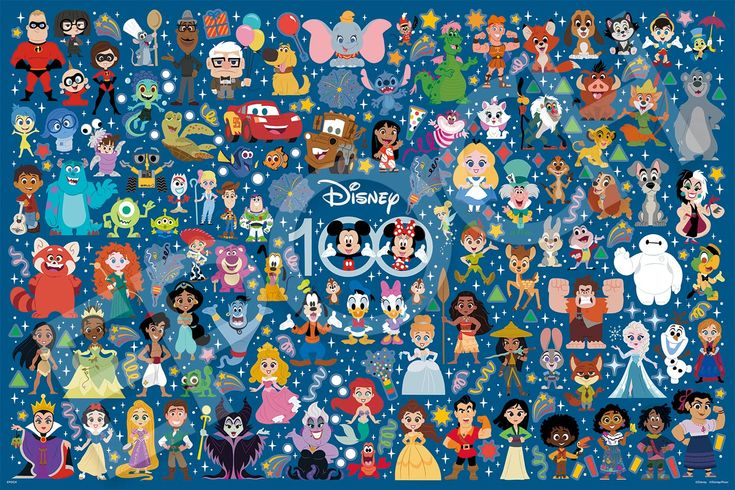
\includegraphics[width=\textwidth]{Graphics/disney.jpeg}
		\caption*{Imagen 1: Disney}
	\end{minipage}
	\hfill
	\begin{minipage}[b]{0.3\textwidth}
		\centering
		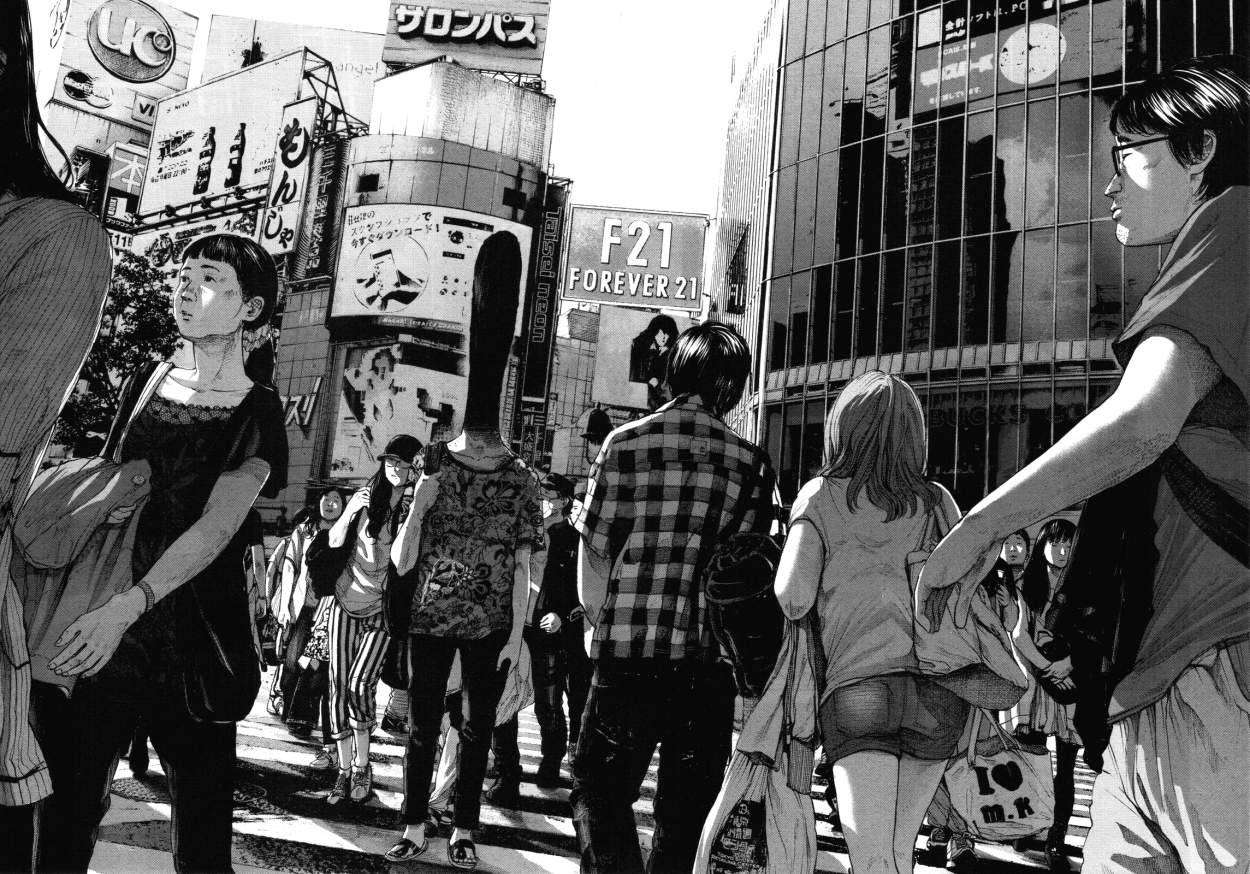
\includegraphics[width=\textwidth]{Graphics/japan.jpg}
		\caption*{Imagen 2: Japan}
	\end{minipage}
	\hfill
	\begin{minipage}[b]{0.3\textwidth}
		\centering
		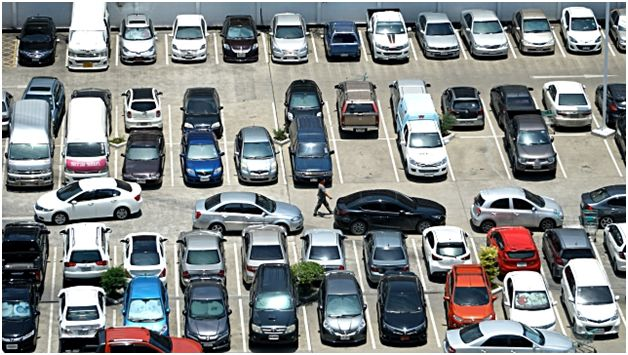
\includegraphics[width=\textwidth]{Graphics/cars.jpeg}
		\caption*{Imagen 3: Cars}
	\end{minipage}
	\caption{Imágenes disponibles para selección en el sistema}
	\label{fig:imagenes-sistema}
\end{figure}

La Tabla \ref{tab:uso-imagenes} muestra la distribución real del uso de imágenes según los datos de 33 usuarios. Se observa una preferencia notable por la imagen Disney (39.39\%), mientras que Japan y Cars presentan una distribución equitativa.


\begin{table}[ht]
	\centering
	\caption{Distribución de uso de imágenes en contraseñas (n = 33)}
	\label{tab:uso-imagenes}
	\begin{tabularx}{0.8\textwidth}{Xcc}
		\toprule
		\textbf{Imagen} & \textbf{Contraseñas} & \textbf{Frecuencia Relativa} \\
		\midrule
		Disney & 13 & 39.39\% \\
		Japan & 10 & 30.30\% \\
		Cars & 10 & 30.30\% \\
		\bottomrule
	\end{tabularx}
	\vspace{0.2cm}

\end{table}



\subsection{Captura de los puntos}
Para seleccionar los puntos se coloca la imagen seleccionada por el usuario de entre un conjunto prove\'ido por el sistema. De esta imagen se obtienen su tama\~no y posicion en la pantalla, de tal manera que al reacionar al evento de click del usuario se pueda calcular la regi\'on de la imagen que haya sido clickada, esto se puede entender de los ejemplos \ref{point-capture1} y \ref{point-capture2} . \\\\

\begin{lstlisting}[ language=Java, caption=C\'odigo de selecci\'on de coordenadas de pantalla, label=point-capture1][hb]
	//seleccionar la posicion en pantalla de la imagen y su tama\~no
  const { left, top, width, height } =
imagecontainer.value.getBoundingClientRect();
//convertir el punto de coordenadas de pantalla a coordenadas de la pantalla en la imagen (cambiar punto de origen)
indicators.push({
	x: ((event.clientX - left) / width) * 100,
	y: ((event.clientY - top) / height) * 100,
});

\end{lstlisting}


\begin{lstlisting}[style=mystyle, language=Java, caption=C\'odigo de transformaci\'on en coordenadas de imagen, label=point-capture2][hb]
	passwordInfo.points = e.map((point: Point) => {
		const { x, y } = point;
		return {
			x: Math.floor((x / 100) * passwordInfo.image.width),
			y: Math.floor((y / 100) * passwordInfo.image.height),
		};
	});
\end{lstlisting}

\subsection{Registro y autenticaci\'on}
\subsubsection{Proceso de Registro}
Durante la fase de registro, el usuario debe ingresar en dos ocasiones su contraseña gráfica (\textit{PassPoints}). Este mecanismo de doble verificación busca incrementar la memorabilidad de la secuencia de clics. Posteriormente, el sistema realiza una llamada a una \textit{edge function} de Supabase, a la cual se transmiten:

\begin{itemize}
	\item Correo insertado por el usuario
	\item Nombre de usuario digitado
	\item Identificador de la imagen seleccionada
	\item Tolerancia utilizada 
	\item Ancho y alto de la imagen
	\item Coordenadas $(x,y)$ de los puntos seleccionados
\end{itemize}

Esta función se encarga de: 
\begin{enumerate}
	\item Discretizar la imagen, obteniendo los parámetros $\phi$  y $\varphi$ de cada punto.
	\item Generar el \textit{hash} de ambas instancias de la contraseña (original y de confirmación) utilizando el m\'etodo explicado en el cap\'itulo anterior.
	\item Validar la congruencia entre ambos \textit{hashes}.
	\item Utilizar los m\'odulos prove\'idos por Supabase para el registro y autenticaci\'on del usuario usando esta informaci\'on.
\end{enumerate}

Al proceso de hashing se le agrega un n\'umero generado aleatoriamente criptogr\'aficamente seguro. Esto hace que los hashes de contrase\~nas iguales sean diferentes y previene ataques de tio \textit{Rainbow Tables}.

\subsubsection{Mecanismo de Registro}
El módulo de autenticación de Supabase emplea un esquema basado en \textit{JSON Web Tokens (JWT)} para:
\begin{itemize}
	\item Gestionar sesiones de usuario
	\item Verificar identidades en cada solicitud
	\item Mantener integridad en la comunicación cliente-servidor
\end{itemize}

Para integrar el sistema \textit{PassPoints} con este servicio:
\begin{itemize}
	\item Se utiliza el \textit{hash} generado del \textit{Passpoints} como contraseña textual en el registro y autenticaci\'on con Supabase.
	\item Se preserva el requisito de entrada válida de \textit{PassPoints} para autenticaciones futuras
	\item Se garantiza compatibilidad con el flujo estándar de OAuth 2.0, lo cu\'al garantiza que se puedan seguir usando los servicios prove\'idos por Supabase.
\end{itemize}


\begin{table}[ht]
	\centering
	\caption{Estructura de la tabla de usuarios}
	\label{tab:bd-esquema}
	\begin{tabularx}{\textwidth}{lX}
		\toprule
		\textbf{Tabla \texttt{user}} & \textbf{Descripción} \\
		\midrule
		\texttt{id} & Identificador único del usuario (UUID v4) \\
		\texttt{email} & Correo electrónico del usuario (único, formato validado) \\
		\texttt{password\_hash} & Hash de la contraseña gráfica \\
		\texttt{phi\_params} & Parámetros de cuantización espacial (JSON) \\
		\texttt{varphi\_params} & Parámetros de tolerancia (JSON) \\
		\texttt{salt} & Valor aleatorio criptográfico (256 bits) \\
		\texttt{tolerance\_radius} & Radio de tolerancia en píxeles (entero 8-32) \\
	
		\bottomrule
	\end{tabularx}
\end{table}


\begin{table}[ht]
	\centering
	\begin{tabularx}{\textwidth}{lX}
		\toprule
		\textbf{Tabla \texttt{Passwords}} & \textbf{Descripción} \\
		\midrule
		\texttt{user\_id} & Clave foránea a \texttt{user.id} \\
		\texttt{image\_id} & Identificador de la imagen base \\
		\texttt{tolerance} & Radio de tolerancia en píxeles \\
		\texttt{points} & Coordenadas $(x,y)$ en texto claro \\
		\texttt{discretization\_params} & $\phi$ y $\varphi$ en texto claro por cada punto (JSON) \\
		\bottomrule
	\end{tabularx}
\end{table}

\subsubsection{Nota de Seguridad}
La decisión de almacenar en texto claro:
\begin{itemize}
	\item Coordenadas de los puntos.
	\item Parámetros $\phi$ y $\varphi$.
	\item Informaci\'on de la imagen, identificador, ancho, alto.
\end{itemize}

\textbf{Se restringe exclusivamente a fines académicos}. En un entorno productivo se aplicarían las siguientes medidas:
\begin{itemize}
	\item Cifrado AES-256 de todos los parámetros sensibles.
	\item No se guardar\'ian las coordenadas originales de la contrase\~na.
	\item No se guardar\'ia la informaci\'on de la imagen utilizada.
\end{itemize}

\subsection{Proceso de Autenticación}

\subsubsection{Flujo de Autenticación}
Durante la fase de autenticación, el usuario debe:

\begin{enumerate}
	\item Seleccionar la imagen utilizada durante el registro de entre tres opciones presentadas en orden aleatorio.
	\item Ingresar su contraseña gráfica (\textit{PassPoints}) sobre la imagen seleccionada
\end{enumerate}

Este diseño incrementa la conciencia del usuario sobre su elección y reduce la predictibilidad del sistema ante posibles ataques.

\subsubsection{Mecanismos de Seguridad}
El sistema implementa las siguientes protecciones:

\begin{itemize}
	\item \textbf{Ocultamiento de regiones de tolerancia}: Los indicadores visuales (recuadros rojos del tama\~no de la regi\'on de tolerancia) se deshabilitan por defecto para prevenir ataques \textit{shoulder surfing}, aunque el usuario puede habilitarlos.
	\item \textit{Edge function} especializada: Valida las credenciales mediante el flujo:
	\begin{enumerate}
		\item Verificación de existencia del usuario en la base de datos
		\item Recuperación de parámetros almacenados ($\varphi$, valor aleatorio $salt$, tolerancia $tolerance_radius$, y \textit{hash} original), valores de \ref{tab:bd-esquema}
		\item Recomputación del \textit{hash} usando el método de discretización descrito en el Capítulo anterior
		\item Verificaci\'on de la autenticidad de la contrase\~na usando el m\'odulo de autenticaci\'on de Supabase.
	\end{enumerate}
\end{itemize}

\begin{table}[ht]
	\centering
	\caption{Parámetros de verificación en autenticación}
	\label{tab:parametros-verificacion}
	\begin{tabularx}{\textwidth}{lXl}
		\toprule
		\textbf{Parámetro} & \textbf{Descripción} & \textbf{Tipo} \\
		\midrule
		$\varphi$ & Lista de $\phi$, $\varphi$ de los puntos & JSON \\
		$c$ & Valor aleatorio  (\textit{salt}) & CHAR (256) \\
		$t$ & Radio de tolerancia & Entero 32 bits \\
		$h$ & \textit{Hash} & \texttt{CHAR(60)} \\
		\bottomrule
	\end{tabularx}
\end{table}

\subsubsection{Gestión de Sesiones}
El servicio de autenticación de Supabase emplea \textit{JSON Web Tokens (JWT)} para:

\begin{itemize}
	\item Generar credenciales temporales con expiración.
	\item Gestionar la validez de los tokens en cada petici\'on y restringir acceso a los servicion en funci\'on de las pol\'iticas de seguridad definidas.
	\item Almacenar el estado de sesión en \textit{cookies} HttpOnly/Secure de lado del usuario, a trav\'es de uso de su cliente de Javascript en la interfaz.
\end{itemize}

La validación resulta en:
\begin{itemize}
	\item Creación de sesión con \textit{token} de acceso/refresh en caso de ser exitosa.
	\item Entrada de un registro en la tabla \textit{auth-passwords} donde se guardan los puntos usados en el intento de autenticaci\'on y el resultado del mismo.
	\item Entrega al cliente de credenciales y datos de sesi\'on para acceder a su informaci\'on en el sistema.
\end{itemize}

\section{Validaci\'on del sistema}

\subsection{Análisis del Espacio de Contraseñas con Discretización Óptima}
\label{subsec:espacio-contrasenas}

El espacio de contraseñas resultante para el sistema \textit{PassPoints} utilizando discretización óptima se calcula mediante la ecuación propuesta en \cite{birget2006graphical}:

\begin{equation}
	P = \left( \frac{a}{6r} \cdot \frac{b}{6r} \right)^c
	\label{eq:espacio-contrasenas}
\end{equation}

donde los parámetros se definen como:

\begin{table}[ht]
	\centering
	\caption{Parámetros del espacio de contraseñas}
	\label{tab:parametros-espacio}
	\begin{tabularx}{0.9\textwidth}{lXl}
		\toprule
		\textbf{Símbolo} & \textbf{Descripción} & \textbf{Dominio} \\
		\midrule
		$a \times b$ & Dimensiones de la imagen (en píxeles) & $\mathbb{Z}^+ \times \mathbb{Z}^+$ \\
		$c$ & Cantidad de puntos seleccionados & $c \geq 5$ \\
		$r$ & Radio de la región de tolerancia & $r \in [8, 32]$ \\
		\bottomrule
	\end{tabularx}
\end{table}

\vspace{0.5cm}

Esta formulación establece que el espacio de contraseñas efectivo $P$ crece exponencialmente con respecto a:
\begin{itemize}
	\item La relación $\frac{a \cdot b}{(6r)^2}$: Densidad de puntos discretizados por área
	\item El número de puntos $c$: Complejidad combinatoria de la secuencia
\end{itemize}

Para una imagen típica de $1024 \times 768$ píxeles con parámetros $r = 16$ y $c = 5$:

\begin{align*}
	P &= \left( \frac{1024}{6 \cdot 16} \cdot \frac{768}{6 \cdot 16} \right)^5 \\
	&= \left( \frac{1024}{96} \cdot \frac{768}{96} \right)^5 \\
	&= (10.6667 \times 8.0)^5 \\
	&= (85.3333)^5 \\
	&\approx 4.43 \times 10^9 \text{ combinaciones}
\end{align*}

Este resultado demuestra que incluso con discretización espacial, el sistema mantiene un espacio de contraseñas comparable al de contraseñas textuales complejas ($\sim$10 bits de entropía por punto). Lo que hace inviable un atauqe de fuerza bruta.


\subsection{Antaques a Passpoints}
Para llevar a cabo una validaci\'on de seguridad del sistema, se presenta un ataque de diccionario extra\'ido de \cite{van2010purely}. El ataque consiste en generar 3 diccionarios basados en diferentes criterios, como fue presentado en el cap\'itulo anterior.

\subsubsection{Diccionario de ataque basado en detecci\'on de bordes}
Para la detecci\'on de bordes su utiliz\'o el algoritmo de Harris \cite{Harris1988ACC}, para todas las im\'agenes, en \cite{van2010purely} justifican el uso de el m\'etodo de detecci\'on de esquinas con la premisa de que los usuarios tienden a seleccionar los mismos puntos donde haya focos de atenci\'on, para detectar los mismos es necesario encontrar los puntos de mayor contraste respecto al resto de la imagen, los bordes son un ejemplo de esto. El resultado de aplicar esto a las im\'agenes del sistema se puede ver en \ref{fig:images-borders}

\begin{figure}[ht]
	\centering
	\begin{minipage}[hb]{0.3\textwidth}
		\centering
		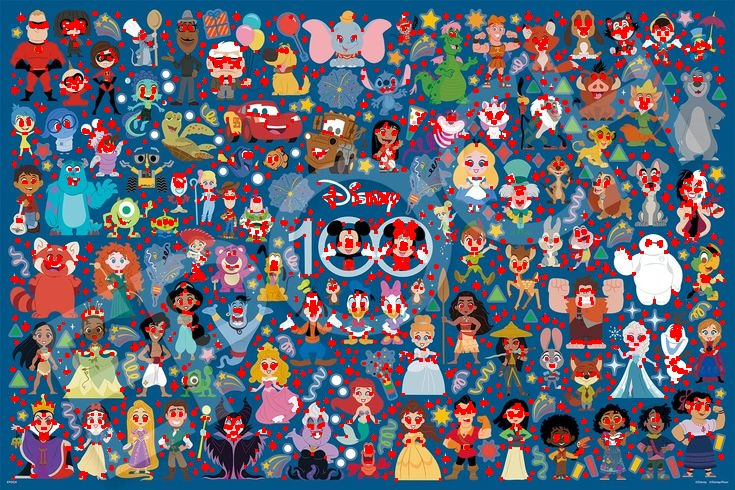
\includegraphics[width=\textwidth]{Graphics/bordes_disney.jpg}
		\captionof*{figure}{Bordes Disney}
	\end{minipage}
	\hfill
	\begin{minipage}[hb]{0.3\textwidth}
		\centering
		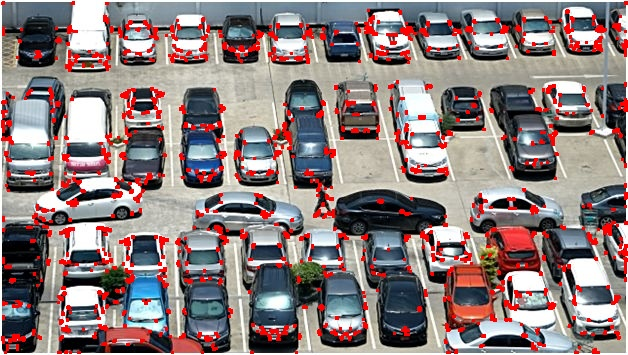
\includegraphics[width=\textwidth]{Graphics/bordes_cars.jpg}
		\captionof*{figure}{Bordes Cars}
	\end{minipage}
	\hfill
	\begin{minipage}[hb]{0.3\textwidth}
		\centering
		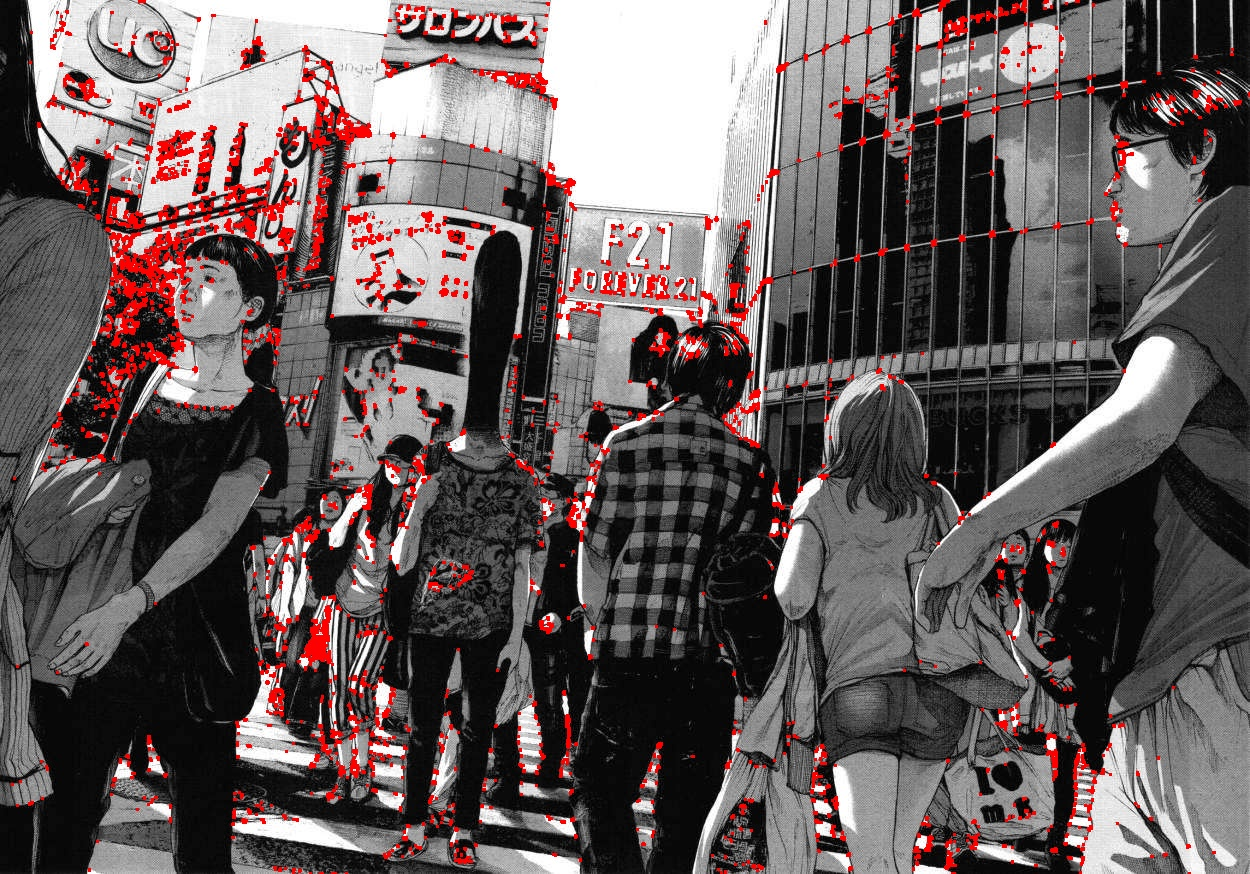
\includegraphics[width=\textwidth]{Graphics/bordes_japan.jpg}
		\captionof*{figure}{Bordes Japan}
	\end{minipage}
	\caption{Imágenes del Sistema con bordes marcados}
	\label{fig:images-borders}
\end{figure}


\subsubsection{Diccionario de ataque basado en segmentaci\'on}
Se segmentaron las im\'agenes y se hall\'o su centro, esto se hizo utilizando el algoritmo \textit{Mean Shift} \cite{Comaniciu2002MeanSA}, de cada segmento tomado se utiliz\'o su centro para crear el diccionario que tuviera en cuento los segmentos en que se divide cada imagen. Visible en figura \ref{fig:images-segments}

\begin{figure}[H]
	\centering
	\begin{minipage}[hb]{0.3\textwidth}
		\centering
		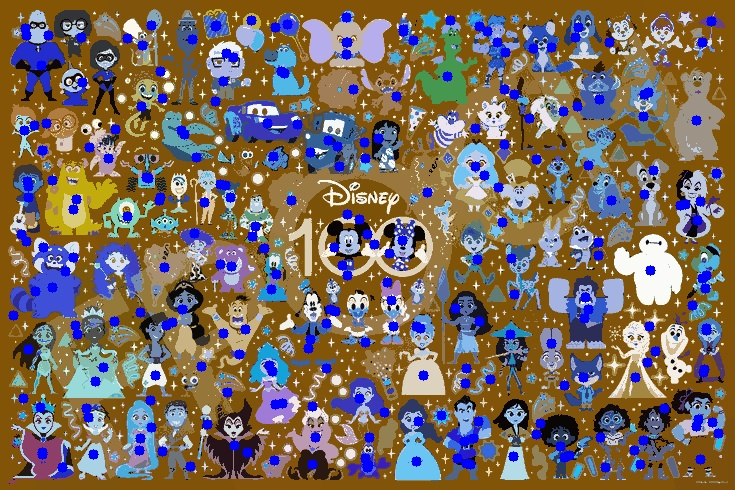
\includegraphics[width=\textwidth]{Graphics/disney-segmented.jpg}
		\captionof*{figure}{Mapa de Segmentaci\'on en imagen Disney}
	\end{minipage}
	\hfill
	\begin{minipage}[hb]{0.3\textwidth}
		\centering
		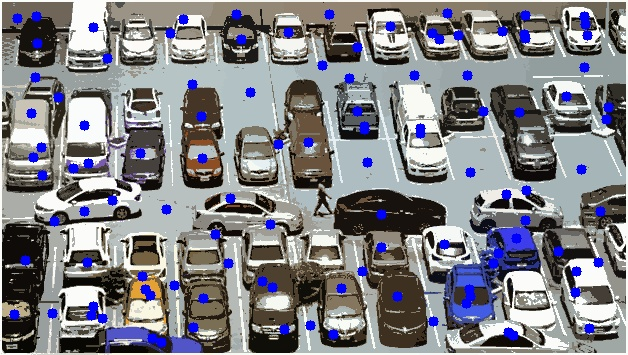
\includegraphics[width=\textwidth]{Graphics/cars-segmented.jpg}
		\captionof*{figure}{Mapa de  segmentaci\'on en imagen Cars}
	\end{minipage}
	\hfill
	\begin{minipage}[hb]{0.3\textwidth}
		\centering
		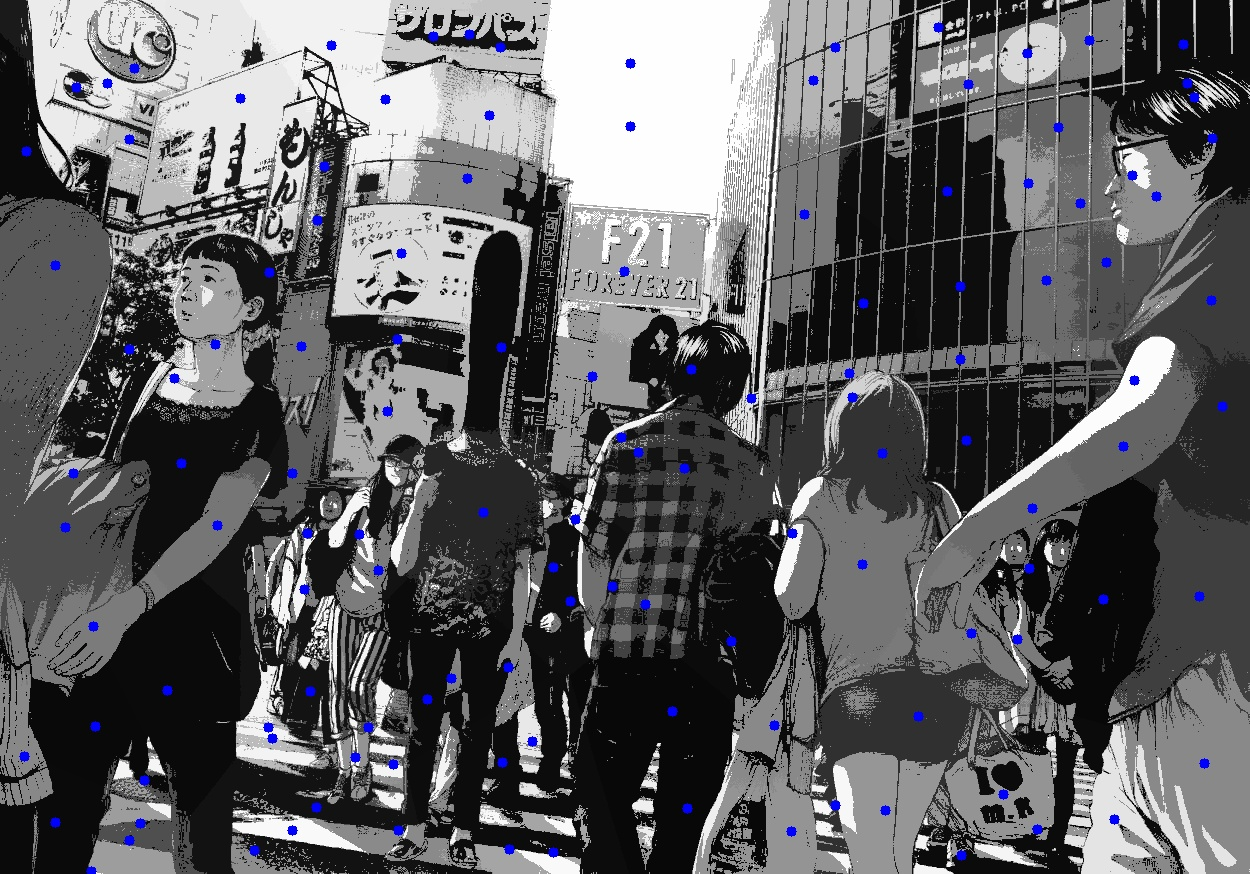
\includegraphics[width=\textwidth]{Graphics/japan-segmented.jpg}
		\captionof*{figure}{Mapa de Segmentaci\'on en imagen Japan}
	\end{minipage}
	\caption{Imágenes del Sistema con sus mapas de segmentaci\'on respectivos y los centros de los mismos marcados}
	\label{fig:images-segments}
\end{figure}

\subsubsection{Diccionario de ataque basado en mapas de atenci\'on visual}
Para calcular los conjuntos de puntos m\'as probables a ser seleccionados por los usuarios se utiliz\'o un modelo de saliencia visual que modela la forma en que los usuarios miran las im\'agenes, el modelo es el propuesto en \cite{itti2000saliency} que es un modelo bottom-up y se basa en caracter\'isticas como el color, direcci\'on que indica cada pixel y su posici\'on en la imagen. Luego de hallar estos mapas se filtr\'o para determinar los puntos que mayor saliencia tuvieran y estos fueron utilizados posteriormente en la generaci\'on de un idccionario de ataque. Se puede visualizar los puntos seleccionados en las figuras \ref{fig:saliency-map} y \ref{fig:selected-points}

\begin{figure}[H]
	\centering
	\begin{minipage}[hb]{0.3\textwidth}
		\centering
		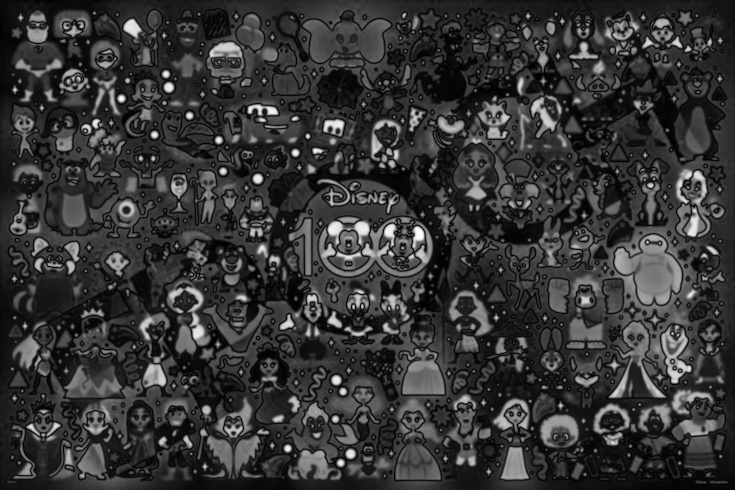
\includegraphics[width=\textwidth]{Graphics/disney-saliency.jpg}
		\captionof*{figure}{Mapa de Atenci\'on en imagen Disney}
	\end{minipage}
	\hfill
	\begin{minipage}[hb]{0.3\textwidth}
		\centering
		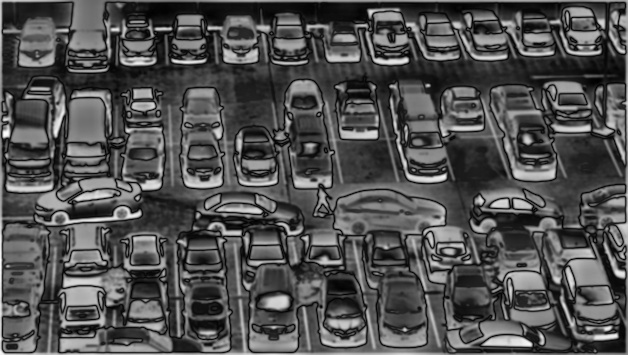
\includegraphics[width=\textwidth]{Graphics/cars-saliency.jpg}
		\captionof*{figure}{Mapa de  Atenci\'on en imagen Cars}
	\end{minipage}
	\hfill
	\begin{minipage}[hb]{0.3\textwidth}
		\centering
		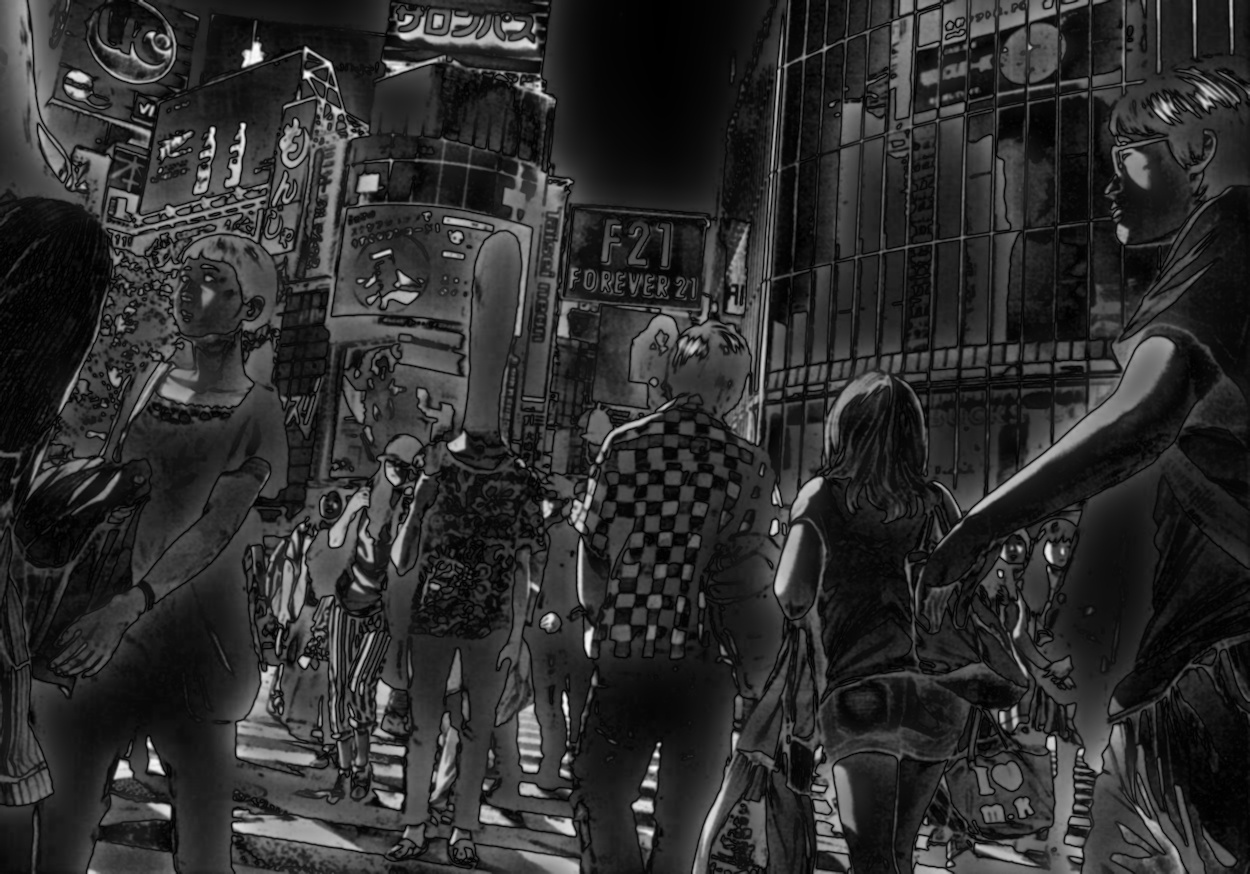
\includegraphics[width=\textwidth]{Graphics/japan-saliency.jpg}
		\captionof*{figure}{Mapa de Atenci\'on en imagen Japan}
	\end{minipage}
	\caption{Imágenes del Sistema con sus mapas de atenci\'on respectivos }
	\label{fig:saliency-map}
\end{figure}

\begin{figure}[H]
	\centering
	\begin{minipage}[hb]{0.3\textwidth}
		\centering
		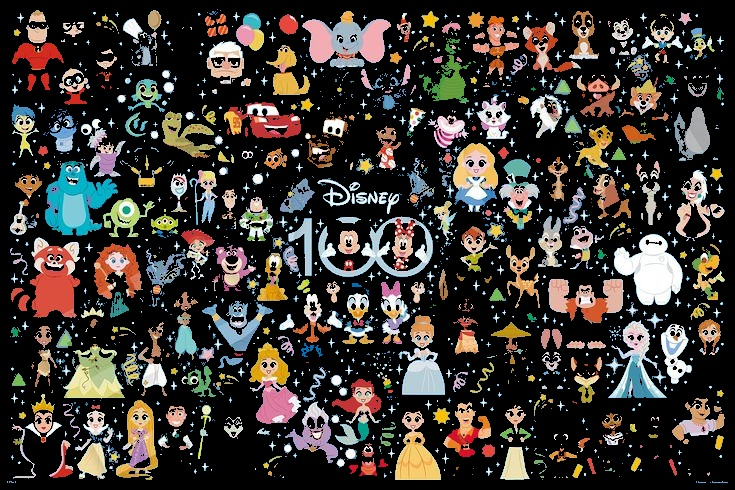
\includegraphics[width=\textwidth]{Graphics/disney-selected-regions.jpg}
		\captionof*{figure}{Regiones seleccionadas en imagen Disney}
	\end{minipage}
	\hfill
	\begin{minipage}[hb]{0.3\textwidth}
		\centering
		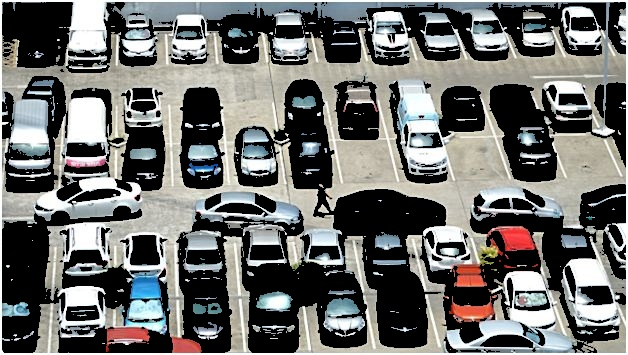
\includegraphics[width=\textwidth]{Graphics/cars-selected-regions.jpg}
		\captionof*{figure}{Regiones seleccionadas en imagen Cars}
	\end{minipage}
	\hfill
	\begin{minipage}[hb]{0.3\textwidth}
		\centering
		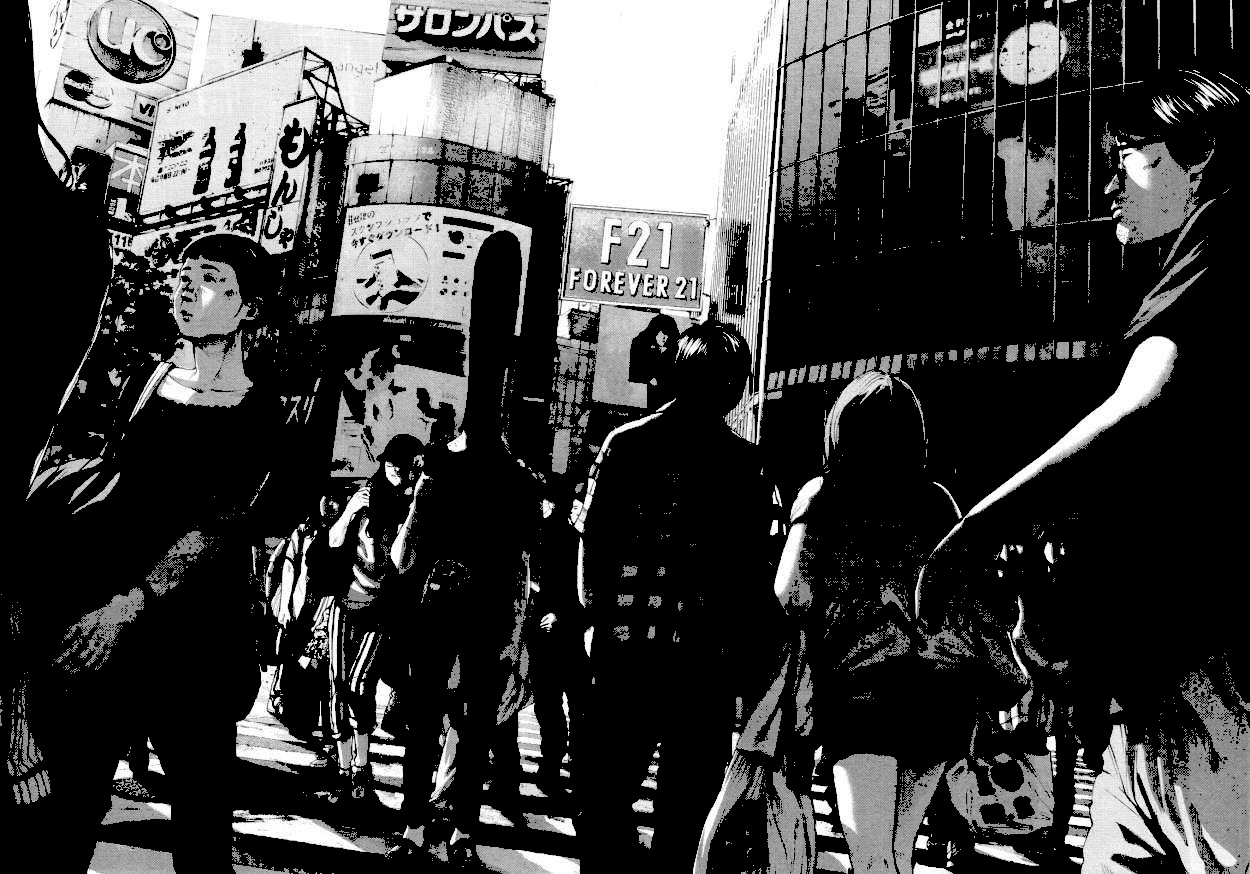
\includegraphics[width=\textwidth]{Graphics/japan-selected-regions.jpg}
		\captionof*{figure}{Regiones seleccionadas en imagen Japan}
	\end{minipage}
	\caption{Imágenes del Sistema con sus respectivas regiones seleccionadas para la creaci\'on del diccionario de ataque}
	\label{fig:selected-points}
\end{figure}


\subsection{Clusterizaci\'on de los puntos }
Para eliminar los puntos que est\'en suficientemente cercanos para caer en la misma regi\'on de tolerancia y reducir las dimensiones de los diccionarios de ataque finales generados, se utiliza el algoritmo de clusterizaci\'on de ventana propuesto en \cite{van2010purely}. Este toma los puntos pertenecientes a una ventana de tama\~no fijo como el mismo, hallando el pixel del centro geom\'etrico de la ventana cada vez. Esto permite eliminar puntos innecesarios y reducir la dimension del espacio de puntos a analizar para generar un diccionario de ataques final. Para estos fines se tom\'o como tama\~no de ventana $3*r$, donde r es el radio de tolerancia de la imagen en p\'ixeles, dando un margen mayor al generado por la regi\'on original que ser\'ia de $2*r$. Esto permiti\'o reducir la cantidad de puntos a analizar, sin perder mucha informaci\'on. En \ref{points:void} se puede ver la cantidad de puntos extra\'idos de cada imagen utilizando las t\'ecnicas de procesamiento anteriormente enunciadas y explicadas, en \ref{points:cluster} se puede observar la reducci\'on sustancial de la cantidad de puntos despu\'es de aplicar el clustering
\begin{table}[!ht]
	\centering
	\caption{Puntos Obtenidos sin clusterizar}
	\label{points:void}
	\begin{tabular}{|l|l|l|l|l|l|l|l|l|l|}
		\hline
		\textbf{imagenes/puntos} & \textbf{segmentos } & \textbf{esquinas} & \textbf{saliencia}
		\\ \hline
		\textbf{disney} & 249 & 30785 & 92981 \\ \hline
		\textbf{cars} & 110 & 17826 & 39764 \\ \hline
		\textbf{japan} & 126 & 47415 & 203804  \\ \hline
	
	\end{tabular}
\end{table}

\begin{table}[!ht]
	\centering
	\caption{Puntos Obtenidos despu\'es de clusterizar}
		\label{points:cluster}
	\begin{tabular}{|l|l|l|l|l|l|l|l|l|l|}
		\hline
		\textbf{imagenes/puntos} & \textbf{segmentos} & \textbf{esquinas} & \textbf{saliencia }  \\ \hline
		\textbf{disney} & 36 & 103 & 65  \\ \hline
		\textbf{cars} & 26 & 98 & 38  \\ \hline
		\textbf{japan} & 30 & 82 & 64 \\ \hline
	\end{tabular}
\end{table}